\chapter*[GERENCIAMENTO DE PROJETO DE SOFTWARE]{GERENCIAMENTO DE PROJETO DE SOFTWARE}

\addcontentsline{toc}{chapter}{GERENCIAMENTO DE PROJETO DE SOFTWARE}
Gerenciar um projeto é aplicar os elementos conhecimentos, habilidades, ferramentas e técnicas às atividades do projeto a fim de atender aos requisitos de negócio. O gerenciamento inclui: identificar requisitos; adaptar às diferentes necessidades à medida que o projeto é planejado e realizado; balancear as restrições conflitantes do projeto que incluem, mas não se limitam a: escopo, qualidade, tempo, custo. \cite{ansi1998}

O empreendimento de um esforço temporário para criar um produto, serviço ou resultado exclusivo é denominado de projeto e possui um fluxo de atividades com início, meio e fim, cujo resultado é único. \cite{pmbok}

A crescente aceitação do gerenciamento de projetos indica que a aplicação desses elementos adequadamente pode ter um impacto significativo no sucesso de um projeto. \cite{pmbok}
A área de gerenciamento de projetos é uma das áreas que mais cresce em utilização no mundo, sendo, hoje, objetivo de investimento em capacitação e metodologia pela maioria das empresas. Em todo projeto, é senso comum que uma das principais dificuldades está na medição e na avaliação dos resultados obtidos, sejam eles resultados finais ou durante sua execução, relacionados a prazos, custos, qualidade, escopo, risco e outros. \cite{vargas2011} \cite{vargas2009}, elucida que a proposta do gerenciamento de projetos é estabelecer um processo estruturado e lógico para lidar com eventos que se caracterizam pela novidade, complexidade e dinâmica ambiental. Um dos fatores que impulsionam o gerenciamento de projetos é o crescimento da competitividade: quem for mais rápido e competente certamente conseguirá os melhores resultados. Essa competividade incita as empresas a conseguirem resultados com menos recursos, em um menor tempo e com mais qualidade.
Perguntas tais como: 1) Quanto tempo levará para desenvolver o software?; 2) Quanto custará o desenvolvimento do software?; dentre outras, são algumas das perguntas as quais todo patrocinador quer saber, pois antes de comprometer os recursos destinados a um projeto, o patrocinador deseja ter uma estimativa de prazo e custo. \cite{pfleeger2004}
Para se aplicar os conceitos de controle de processo faz-se necessário diferenciar duas modalidades, não concomitantes, aplicáveis ao gerenciamento de projetos: metodologia com processo definidos (ou prescritivos) e a metodologia empírica. De acordo com \cite{martins2007}, a primeira define o contexto do projeto e o escopo das entradas logo no início do projeto, enquanto que a outra define as entregas de forma abrangente e superficial, começando por um contexto inicial, que evolui e se adapta ao longo da execução.

\section{GERENCIAMENTO TRADICIONAL}
A metodologia com processos definidos e prescritivos, também chamada de abordagem tradicional, é a mais adequada em situações onde os passos a serem executados, em geral, são conhecidos, como por exemplo, na implantação de uma infraestrutura de TI. Em projetos tradicionais, certo conjunto de entradas produzirá um conjunto específico de saídas. \cite{martins2007}

\subsection{O guia PMBOK}
O Guia PMBOK® fornece diretrizes para o gerenciamento de projetos individuais, define o gerenciamento e os conceitos relacionados, e descreve o ciclo de vida do gerenciamento de projetos e os processos relacionados. Tem por objetivo ser um guia com um conjunto de conhecimentos e boas práticas de aplicação. Não é uma metodologia, é uma referência básica, logo, a norma não é abrangente nem completa, possibilita o uso de ferramentas e metodologias distintas para implementar sua estrutura, e fornece um vocabulário comum para se discutir, escrever e aplicar o gerenciamento de projetos entre os membros envolvidos.
O guia é baseado em várias áreas e processos que organizam o trabalho a ser realizado durante o projeto. Os processos se relacionam e interagem segundo uma lógica definida para a condução do trabalho, realizada através de entradas, ferramentas e técnicas, e saídas.

\subsubsection{Ciclo de vida e a organização do projeto}
Consiste nas fases que oferecem uma estrutura básica para o gerenciamento do projeto, independente do trabalho especifico envolvido, todos os projetos podem ser mapeados para a estrutura do ciclo de vida: 1) Início do projeto; 2) Organização e preparação; 3) Execução do trabalho do projeto; e 4) Encerramento do projeto.  Esta estrutura pode ser visualizada na Figura 1(PMI, 2008).

\begin{figure}[!htb]
\centering
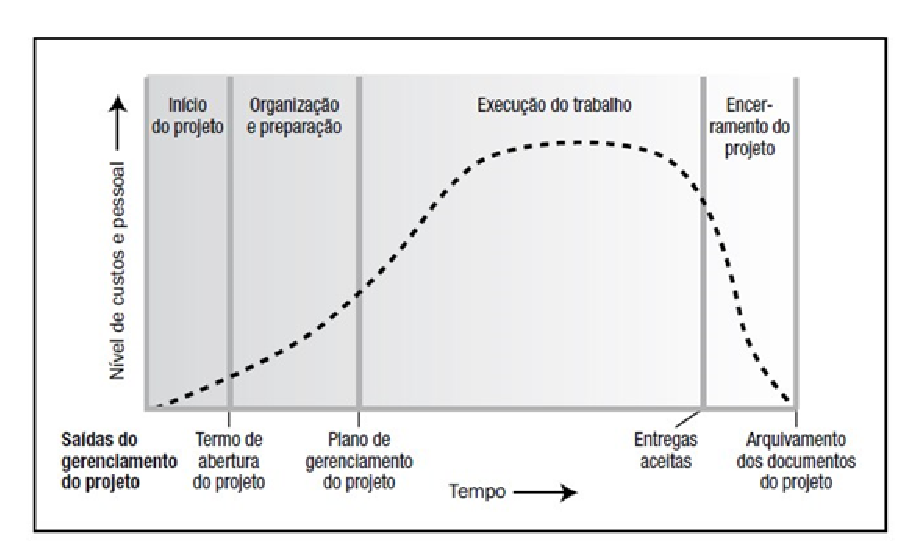
\includegraphics{figuras/fig1.eps}
\caption{ Nível típico de custos e pessoal ao longo do seu ciclo de vida. Fonte \cite{pmbok}}
\label{fig1}
\end{figure}



